There are many ways to design and implement applications for a distributed cluster, a set of
computers (typically labeled as \emph{computing nodes}) that have their own independent
processors and memory, and are connected together with a computer network. In the context of
\gls{hpc}, such distributed clusters are called \emph{supercomputers}, and
one of their distinguishing features is that all the computers of the cluster reside within one
physical location, and they are connected with a very high-speed and low-latency network
connection. There are also many other kinds of distributed clusters, such as data centers or
cloud-based distributed systems, however this thesis focuses almost exclusively on
\gls{hpc} systems and supercomputers.

Distributed applications are implemented using various \emph{programming models}, which should be
able to provide a way to efficiently utilize the available computing resources of the cluster, and
to allow expressing communication patterns that enable the individual cluster nodes to cooperate
and exchange data. Communication between nodes is crucial, as that is what allows distributed
clusters to offer unparalleled performance by distributing the computational load amongst multiple
computers and thus achieving speedup through parallelization.

There are many different programming models and tools for creating distributed applications, and it
can be challenging to understand how do they relate to one another. It is especially difficult to
navigate the area of \emph{task-based programming}, which is the main focus of this thesis, because
common umbrella terms like \emph{task}, \emph{task graph},
\emph{\gls{dag}}, \emph{workflow} or \emph{pipeline} are being
used very liberally, and they can represent vastly different concepts. It is thus possible to
encounter two programming models or tools that both claim to use ``task-based programming'', even
though they might have very little in common.

This chapter provides a broad overview of the most popular approaches for implementing distributed
and parallel applications, with the focus on \gls{hpc} use-cases. It describes
both various programming models and also state-of-the-art tools that leverage them. It categorizes
these tools based on several properties, and gradually concretizes which niches of this diverse
area are most relevant for the topic of this thesis.

\section{Parallel programming models}
This section describes the most important representatives of programming models that are used in
the world of supercomputing. It divides the programming models into two broad categories; models
that express parallelization and network communication explicitly, and models that do so
implicitly.

\subsection*{Explicit parallelization}
One way to design distributed applications is to leverage programming models that express the
parallelization of computation and the exchange of data between nodes explicitly. This has been the
predominant way of creating \gls{hpc} software for many years, and it is still
very popular today~\cite{mpiusagestudy1,mpiusagestudy2,mpiusagestudy3}. Below are a few examples of these explicit
approaches.

\begin{description}
	\item[Message passing] has historically been the most popular method for implementing \gls{hpc} software.
		In this model, a distributed computation is performed by a set of processes with separate memory
		address spaces that are running on independent computing nodes. The processes cooperate together to
		solve complex problemss by exchanging network messages (hence the term \emph{message passing}).
		Message passing applications are commonly implemented using the
		\gls{spmd}~\cite{spmd} computational model, where the implementation
		logic of all the processes participating in the computation is embedded within a single program.

		The most popular representative of this programming model is the
		\gls{mpi}~\cite{mpi} framework, which is used by a large amount of
		existing \gls{hpc} applications~\cite{mpiusagestudy2}. It defines a set of
		communication primitives, operators and data types, which can be used to perform computations,
		exchange data and synchronize progress between either two (\emph{point-to-point communication}) or multiple
		(\emph{collective communication}) processes running on distributed nodes. \Autoref{lst:mpi-example}
		shows a simple \gls{mpi} program which is designed to execute on two (potentially
		distributed) processes. The first process sends a number to the second process, which waits until
		that number is received, and then prints it to standard output. Notice how both network
		communication and synchronization is expressed explicitly, by calling the
		\texttt{MPI\_Send} and \texttt{MPI\_Recv} functions. We can also see the
		\gls{spmd} paradigm in practice, because the code for both processes is interleaved
		within the same program.

		\begin{listing}[h]
			\caption{Simple \gls{mpi} program implemented in \texttt{C}}
			\label{lst:mpi-example}
			\begin{minted}[fontsize=\small]{c}
	#include <mpi.h>
	#include <stdio.h>

	int main() {
		MPI_Init(NULL, NULL);

		// Find out the ID of this process
		int process_id;
		MPI_Comm_rank(MPI_COMM_WORLD, &process_id);

		if (process_id == 0) {
			// Send one integer to process 1
			int value = 42;
			MPI_Send(&value, 1, MPI_INT, 1, 0, MPI_COMM_WORLD);
		} else if (process_id == 1) {
			// Receive one integer from process 0
			int value = 0;
			MPI_Recv(&value, 1, MPI_INT, 0, 0, MPI_COMM_WORLD, MPI_STATUS_IGNORE);
			printf("Process 1 received number %d from process 0\n", value);
		}

		MPI_Finalize();

		return 0;
	}
				  \end{minted}
		\end{listing}

	\item[\gls{pgas}~\cite{pgas}] is a relatively similar programming model, which also often employs the \gls{spmd}
		paradigm. Where it differs from message passing is in the way it expresses communication between
		processes. Message passing processes share their memory by communicating with other processes,
		while PGAS provides an abstraction of a shared memory address space and allows processes to
		communicate through it\footnote{To paraphrase the famous ``Do not communicate by sharing memory; instead, share memory by communicating'' quote coined by the \texttt{Go} programming
		language.}. \gls{pgas} provides an illusion
		of a global memory address space that is available to processes that participate in the
		communication, which makes it slightly less explicit in terms of expressing the communication
		patterns within the program, because it translates certain memory operations into network messages
		on behalf of the programmer.

		\gls{pgas} programs also often employ \emph{one-sided communication} techniques, such
		as \gls{rdma}, which allows a process to directly read or write a region of memory
		from the address space of a different process.

	\item[Shared-memory multiprocessing] is an approach that focuses on the parallelization within a single computing node, by leveraging
		multithreading to achieve speedup. In the area of \gls{hpc}, it is common to use
		the \gls{openmp}~\cite{openmp} framework to implement multithreaded
		applications. Apart from providing interfaces for parallelizing code, synchronizing threads through
		barriers or various locks, or performing atomic operations, it is also able to offload computation
		to various accelerators (like a \gls{gpu}) attached to the node.
		\gls{openmp} can be used together with the two previously mentioned programming
		models (it is often combined especially with
		\gls{mpi}~\cite{hybrid_openmp_mpi}), in order to achieve parallelization both
		intra-node (via multithreading) and inter-node (via network communication).

		\gls{openmp} does not only offer an \gls{api}, but it can also be
		integrated directly within a compiler, e.g.\ in \gls{gcc} for programs written in
		the \texttt{C} or \texttt{C++} programming languages. This enables it
		to provide source code annotations (called \emph{pragmas}), which allow the programmer
		to parallelize a region of code with very little effort. An example of this can be seen in
		\Autoref{lst:openmp-annotation}, where a loop is parallelized simply by adding a single annotation to
		the source code.

		\begin{listing}
			\caption{Simple \gls{openmp} annotation}
			\label{lst:openmp-annotation}
			\begin{minted}[fontsize=\small]{c}
void compute_parallel(int* items, int count) {
    // This loop is executed in parallel
    #pragma omp parallel for
    for (int i = 0; i < count; i++) {
        items[i] = compute(i);
    }
}
        \end{minted}
		\end{listing}
\end{description}

These explicit programming models share a lot of desirable properties. They give their users a lot
of control over the exchange of data between individual cores and distributed nodes, which allows
creating very performant programs. Having the option to explicitly describe how will the individual
cores and nodes cooperate also enables expressing arbitrarily complex parallelization patterns and
data distribution strategies. However, in order to fully exploit the performance potential of
explicit parallelization, the programmer must have advanced knowledge of the
\gls{cpu} or \gls{gpu} hardware
micro-architecture~\cite{intel_developer_manual} and the memory model of the used programming
language~\cite{cpp11_standard}.

Even though explicitly parallelized programs can be incredibly efficient, implementing correct
applications using them is notoriously difficult. Multithreaded and distributed programs are highly
concurrent, which makes it easy to introduce various programming errors, such as deadlocks, race
conditions or data races. Especially for distributed programs, debugging such issues can be
incredibly challenging. Furthermore, programs that leverage explicitly parallel programming models
are typically implemented in languages such as \texttt{C} or
\texttt{C++}, which are infamous for making it difficult to write correct,
memory-safe programs without memory errors and undefined behaviour~\cite{memory_safety_report}.
Memory safety issues are even more problematic in heavily concurrent programs, which further
increases the difficulty and decreases the speed of developing correct distributed programs.

Apart from correctness, using explicit communication interfaces can also lead to overdependence on
a specific state of available computational resources. For example, \gls{mpi}
programs typically assume a fixed number of processes participating in the computation, and
\gls{mpi} itself struggles with situations where some of the processes
participating in the computation crash or disappear, which infamously makes it challenging to
implement fully fault-tolerant \gls{mpi} programs~\cite{fault_tolerant_mpi}.

\subsection*{Implicit parallelization}
Since it can take a lot of effort to implement a correct and efficient distributed program using
explicitly parallel models, it would be unreasonable to expect that all users who want to leverage
\gls{hpc} resources to execute their experiments will ``roll up their sleeves''
and spend months implementing an explicitly parallel \texttt{C++} program that uses
\gls{mpi} and \gls{openmp}. In fact, with scientific experiments
becoming more and more complex each year, in most cases it would not even be feasible to develop
custom (explicitly parallel) code for them from scratch. Instead, high-performance parallelized
primitives implemented by specialized performance engineers~\cite{dace} are moving
into libraries and frameworks, such as GROMACS~\cite{gromacs,gromacs_mpi} or
TensorFlow~\cite{tensorflow,horovod}, that still leverage technologies like
\gls{mpi} or \gls{openmp} internally, but they do not necessarily
expose them to their end users.

This allows users of \gls{hpc} systems and scientists to focus on their problem
domain, as their responsibility shifts from implementing communication and parallelization
techniques by hand to describing high-level computational workflows using
\emph{implicity parallel} programming models that are able to automatically derive the
communication and parallelization structure from the program description. With an implicitly
parallel model, the emphasis moves from \emph{how} to perform a distributed or
parallelized computation (which is the essence of the explicit models) to
\emph{what} should be computed and how are the individual computational steps
related to each other, which is usually the main aspect that users actually want to focus on.
Implicitly parallel programming models often combine aspects of two programming paradigms,
declarative and imperative. The possible parallelization opportunities are expressed using
declarative approaches, for example using various \glspl{dsl}, while sequential
parts of code usually remains imperative.

The primary benefit of the implicitly parallel approaches is that they make it easy to define a
computation that can be automatically parallelized, without forcing the user to think about how
exactly will the parallelization and network communication be performed. Execution frameworks are
then able to ingest programs implemented with implicitly parallel models and automatically execute
them on a parallel machine or even a distributed cluster in a parallel fashion, thus making it much
easier for the user to leverage available hardware resources. Implicit models are easier to use
than the explicit models, and they facilitate rapid prototyping of parallelized programs.

On the other hand, the main disadvantage of these models is the lack of control of how exactly is
parallelization performed. Therefore, programs implemented using them might not be able to achieve
the same performance as explicitly parallelized programs.

There are various models that support implicit parallelization, for example stencil
computations~\cite{stencil} or automatically parallelized functional
languages~\cite{parallel_haskell}. But by far the most popular are the many tools and models
based on tasks. Since task-based programming is a core topic of this thesis, the rest of the thesis
will focus exclusively on programming models that leverage tasks. In particular, the following
section will categorize these models based on several properties, and describe representative tools
that implement this paradigm.

\section{Computational workflows}
In recent years, it became very popular to define scientific computations running on distributed
and \gls{hpc} clusters using
\emph{task-based programming models}~\cite{pegasus,workflows1,workflows_at_scale}. These models allow their users to describe
the high-level structure of their computations using \emph{computational workflows} (also called \emph{pipelines} or \emph{task graphs}\footnote{These three terms will be used interchangeably in this thesis.}). A computational
workflow is a \gls{dag} of \emph{tasks}, atomic and independent
computational blocks with separate inputs and outputs that can depend on one another, which can be
executed in a self-contained way. Such workflows can naturally express diverse scientific
experiments, which typically need to execute and compose many independent steps with dependencies
between themselves (for example data preprocessing, postprocessing and analysis computations,
various simulations, etc.). They are also very flexible and easy to use, which is what makes them
popular.

Since task-based programming models are implicitly parallel, their users do not have to
imperatively specify how should their computation be parallelized, or when and how should data be
exchanged between distributed nodes. They merely declaratively describe the individual parts of the
program that can theoretically be executed in parallel (the tasks) and then pass the task graph to
a dedicated execution tool (that we will label as a \emph{task runtime}) that executes the
tasks, typically on a distributed cluster. Since the program is represented with an explicit graph,
the taks runtime can effectively analyze its properties (or even optimize the structure of the
graph) in an automated way, and extract the available parallelism from it without requiring the
user to explicitly define how should the program be parallelized.

It is important to note that from the perspective of a taks runtime, each task is opaque. The tool
knows how to execute it, but it typically does not have any further knowledge of the inner
structure of the task. Therefore, the only parallelization opportunities that can be extracted by
the tool have to be expressed by the structure of the task graph. A task graph containing a single
task is thus not very useful on its own. The individual tasks can of course also be internally
parallel, however this parallelization is not provided automatically by the task runtime. Tasks
often achieve internal parallelism using shared memory multiprocessing, for example using the
\gls{openmp} framework.

Since task-based programming models are quite popular, there are hundreds of different tools and
technologies that leverage them. It can be challenging to understand how do these tools relate to
one another, because umbrella terms like \emph{task}, \emph{task graph},
\emph{\gls{dag}}, \emph{workflow} or \emph{pipeline} can
represent vastly different concepts in different contexts. For example, the term task is used for
many unrelated concepts in computer science, from an execution context in the Linux kernel, through
a block of code that can be executed on a separate thread by \gls{openmp}, to a
program that is a part of a complex distributed computational workflow. It is thus possible to
encounter two programming models or tools that both claim to use ``task-based programming'', even
though they might have very little in common. The rest of this section will thus categorize
existing state-of-the-art tools that use task-based programming models based on several properties,
to put them into a broader context, and it will also gradually specify which niches of this diverse
area are most relevant for the topic of this thesis.

\subsection*{Batch vs stream processing}
One of the most distinguishing properties that divides distributed task processing tools into two
broad categories is the approach used to trigger the execution of the workflow.
\emph{Stream processing} tools are designed to execute continuously, and react to external
events that can arrive asynchronously and at irregular intervals, while typically focusing on low
latency. A streaming computational workflow is executed every time a specific event arrives. The
workflow can then can analyze the event, and generate some output, which is then e.g.\ persisted in
a database or sent to another stream processing system. As an example, a web application can stream
its logs, which are being generated dynamically as users visit the website, to a stream processing
tool, which then analyzes the logs and extracts information out of them in real-time. Popular
representatives of stream processing are for example Apache Flink~\cite{flink} or
Apache Kafka~\cite{kafka}. Streaming-based tools can also be implemented using the
\emph{dataflow} programming model~\cite{dataflow,timely_dataflow}.

In contrast, \emph{batch processing} tools are designed to perform a specific computation over
a set (batch) of input data that is fully available before the computation starts, while focusing
primarily on maximal throughput. Such workflows are usually triggered manually by a user once all
the data is prepared, and the workflow stops executing once it has processed all of its inputs. In
certain cases, parts of the computation can be generated dynamically, while the workflow is already
executing. For example, iterative workflows perform a certain computation repeatedly in a loop,
until some condition in met. Typical representatives of batch processing tools are for example
\dask{}~\cite{dask}, SnakeMake~\cite{snakemake} or
SciLuigi~\cite{sciluigi}.

Streaming processing is common in the area of cloud computing, and is useful especially for
analyzing data that is being generated in real-time. It is not very common in the world of
supercomputing though, because \gls{hpc} hardware resources are typically
ephemeral, and they are not designed to be available for a single user at all times, which limits
their usefulness for handling real-time events that occur at unpredictable times. On the other
hand, batch processing workflows are a better fit for \gls{hpc} clusters, since
their execution time is bounded by the size of their input, which is often known in advance, and
thus they can be more easily mapped to ephemeral, time-limited allocations of
\gls{hpc} hardware resources. This thesis thus exclusively focuses on batch
processing.

\subsection*{Task graph generality}
Even though basically all workflow processing tools are designed to execute a
\gls{dag} of tasks, not all of them support arbitrary task graphs. Some tools use
programming models designed for specialized use-cases, which allows them to offer very high-level
and easy-to-use \glspl{dsl} and \glspl{api} that are designed to
perform a specific set of things well, but that do not allow expressing fully general task graphs.

An example of such a constrained approach is the Bulk synchronous
parallel~\cite{bulkparallel1} model, which models a distributed computation with a series of
steps that are executed in order. Within each step, a specific computation is performed in
parallel, potentially on multipled distributed nodes. At the end of each step, the nodes can
exchange data amongst themselves, and they are synchronized with a global barrier, to ensure that
there are no cyclic communication patterns in the computation. Even though this model does not use
fully arbitrary computational graphs, it is still possible to express many algorithms with
it~\cite{bulkparallel2}.

A popular instance of this model that has gained a lot of popularity in the area of distributed
computing is MapReduce~\cite{mapreduce}. Its goal is to allow parallel processing of
large amounts of data on a distributed cluster in a fault-tolerant way, while providing a simple
interface for the user. It does that by structuring the computation into three high-level
operations, which correspond to individual bulk synchronous parallel steps:
\begin{enumerate}
	\item A \emph{map} operation (provided by the user) is performed on the input data. This
	      operation performs data transformation and filtering, associates some form of a
	      \emph{key} to each data item and produces a key-value tuple.
	\item A \emph{shuffle} operation (implemented by a MapReduce framework) redistributes the
	      tuples amongst a set of distributed nodes, based on the key of each tuple, so that tuples with the
	      same key will end up at the same node.
	\item A \emph{reduce} operation (provided by the user) is performed on each node. The
	      reduction typically performs some aggregation operation (such as sum) on batches of tuples, where
	      each batch contains tuples with the same key.
\end{enumerate}

This approach is an instance of the \emph{split-apply-combine}~\cite{split_apply_combine}
paradigm, which describes the following intuitive strategy for parallel computations on a dataset:
\emph{split} the data into multiple chunks, \emph{apply} some
transformation to each chunk in parallel (this corresponds to the \emph{map}
operation) and then \emph{combine} the results (this corresponds to the
\emph{reduce} operation).

\begin{listing}
	\caption{MapReduce word count implemented in Python}
	\label{lst:wordcount-example}
	\begin{minted}[fontsize=\small, tabsize=4]{python}
def word_count(context):
	file = context.textFile("shakespeare.txt")
	counts = file.flatMap(lambda line: line.split(" ")) \
		.map(lambda word: (word, 1)) \
		.reduceByKey(lambda x, y: x + y)
	output = counts.collect()
	print(output)
	\end{minted}
\end{listing}

\Autoref{lst:wordcount-example} shows a simple Python program that computes the frequency of
individual words in a body of text\footnote{This computation is commonly known as \emph{word count}.} using a popular implementation of
MapReduce called Apache Spark~\cite{spark}. Even though the programmer only needs to
provide a few simple \emph{map} and \emph{reduce} operations, this
short program can be executed on a distributed cluster and potentially handle large amounts of
data. Note that multiple \emph{map} and \emph{reduce} operations can
be combined in a single program, which can also be observed in this example. While this program is
implemented in the Python programming language, the most important parts of the computation are
expressed using a few very specific implicitly parallel operations (\emph{map} and
\emph{reduce}), therefore it is possible to consider this to be a sort of
\gls{dsl} for expressing distributed computations.

The primary benefit of this approach is that it is quite easy to define a computation that can be
automatically parallelized and distributed. Furthermore, the ``layered'' shape of task graphs
produced by MapReduce programs facilitates implementation of fault tolerance, because there are
clearly delimited checkpoints where the intermediate results of the computation can be persisted to
disk (at the end of each \emph{map} or \emph{reduce} operation), so
that they can be later restored in case of failure. This is only possible because the tools that
execute MapReduce programs have additional knowledge and invariants about the shape of the task
graph, due to its constrained nature.

However, this is also the main limitation of this model. If a computation cannot be naturally
expressed using the \emph{map} and \emph{reduce} operations, it can
be challenging, or even impossible, to implement it with the MapReduce paradigm. In particular,
MapReduce assumes forward data-flow, where data is being sent through the computational pipeline in
one direction. This can be problematic for iterative computations that have to execute repeatedly,
e.g.\ until some condition is reached, and which typically use the output of a previous iteration
as an input for the next iteration, thus creating a loop in the flow of data.

An additional potential disadvantage, which is shared by most implicitly parallel models, is that
MapReduce programs might not be able to achieve performance comparable to programs implemented
using explicit parallelism. This is especially problematic for certain implementations of MapReduce
that are known to be very inefficient, such as Apache Hadoop~\cite{hadoop}. In
general, when executing distributed computations, it is always a good idea to first make sure that
it is not possible to solve the same problem faster with a single-threaded program running on
consumer-grade hardware~\cite{cost}.

\begin{listing}[h]
	\caption{\dask{} DataFrame query and its corresponding task graph}
	\label{lst:dask-dataframe-example-1}
	\begin{minipage}{.4\linewidth}
		\begin{minted}[fontsize=\small, tabsize=4]{python}
import dask.dataframe as pd

df = pd.read_csv("dataset.csv")
# This query is translated to the
# task graph shown on the right
df.groupby("Country").GDP.mean()
	\end{minted}
	\end{minipage}
	\begin{minipage}{.6\linewidth}
		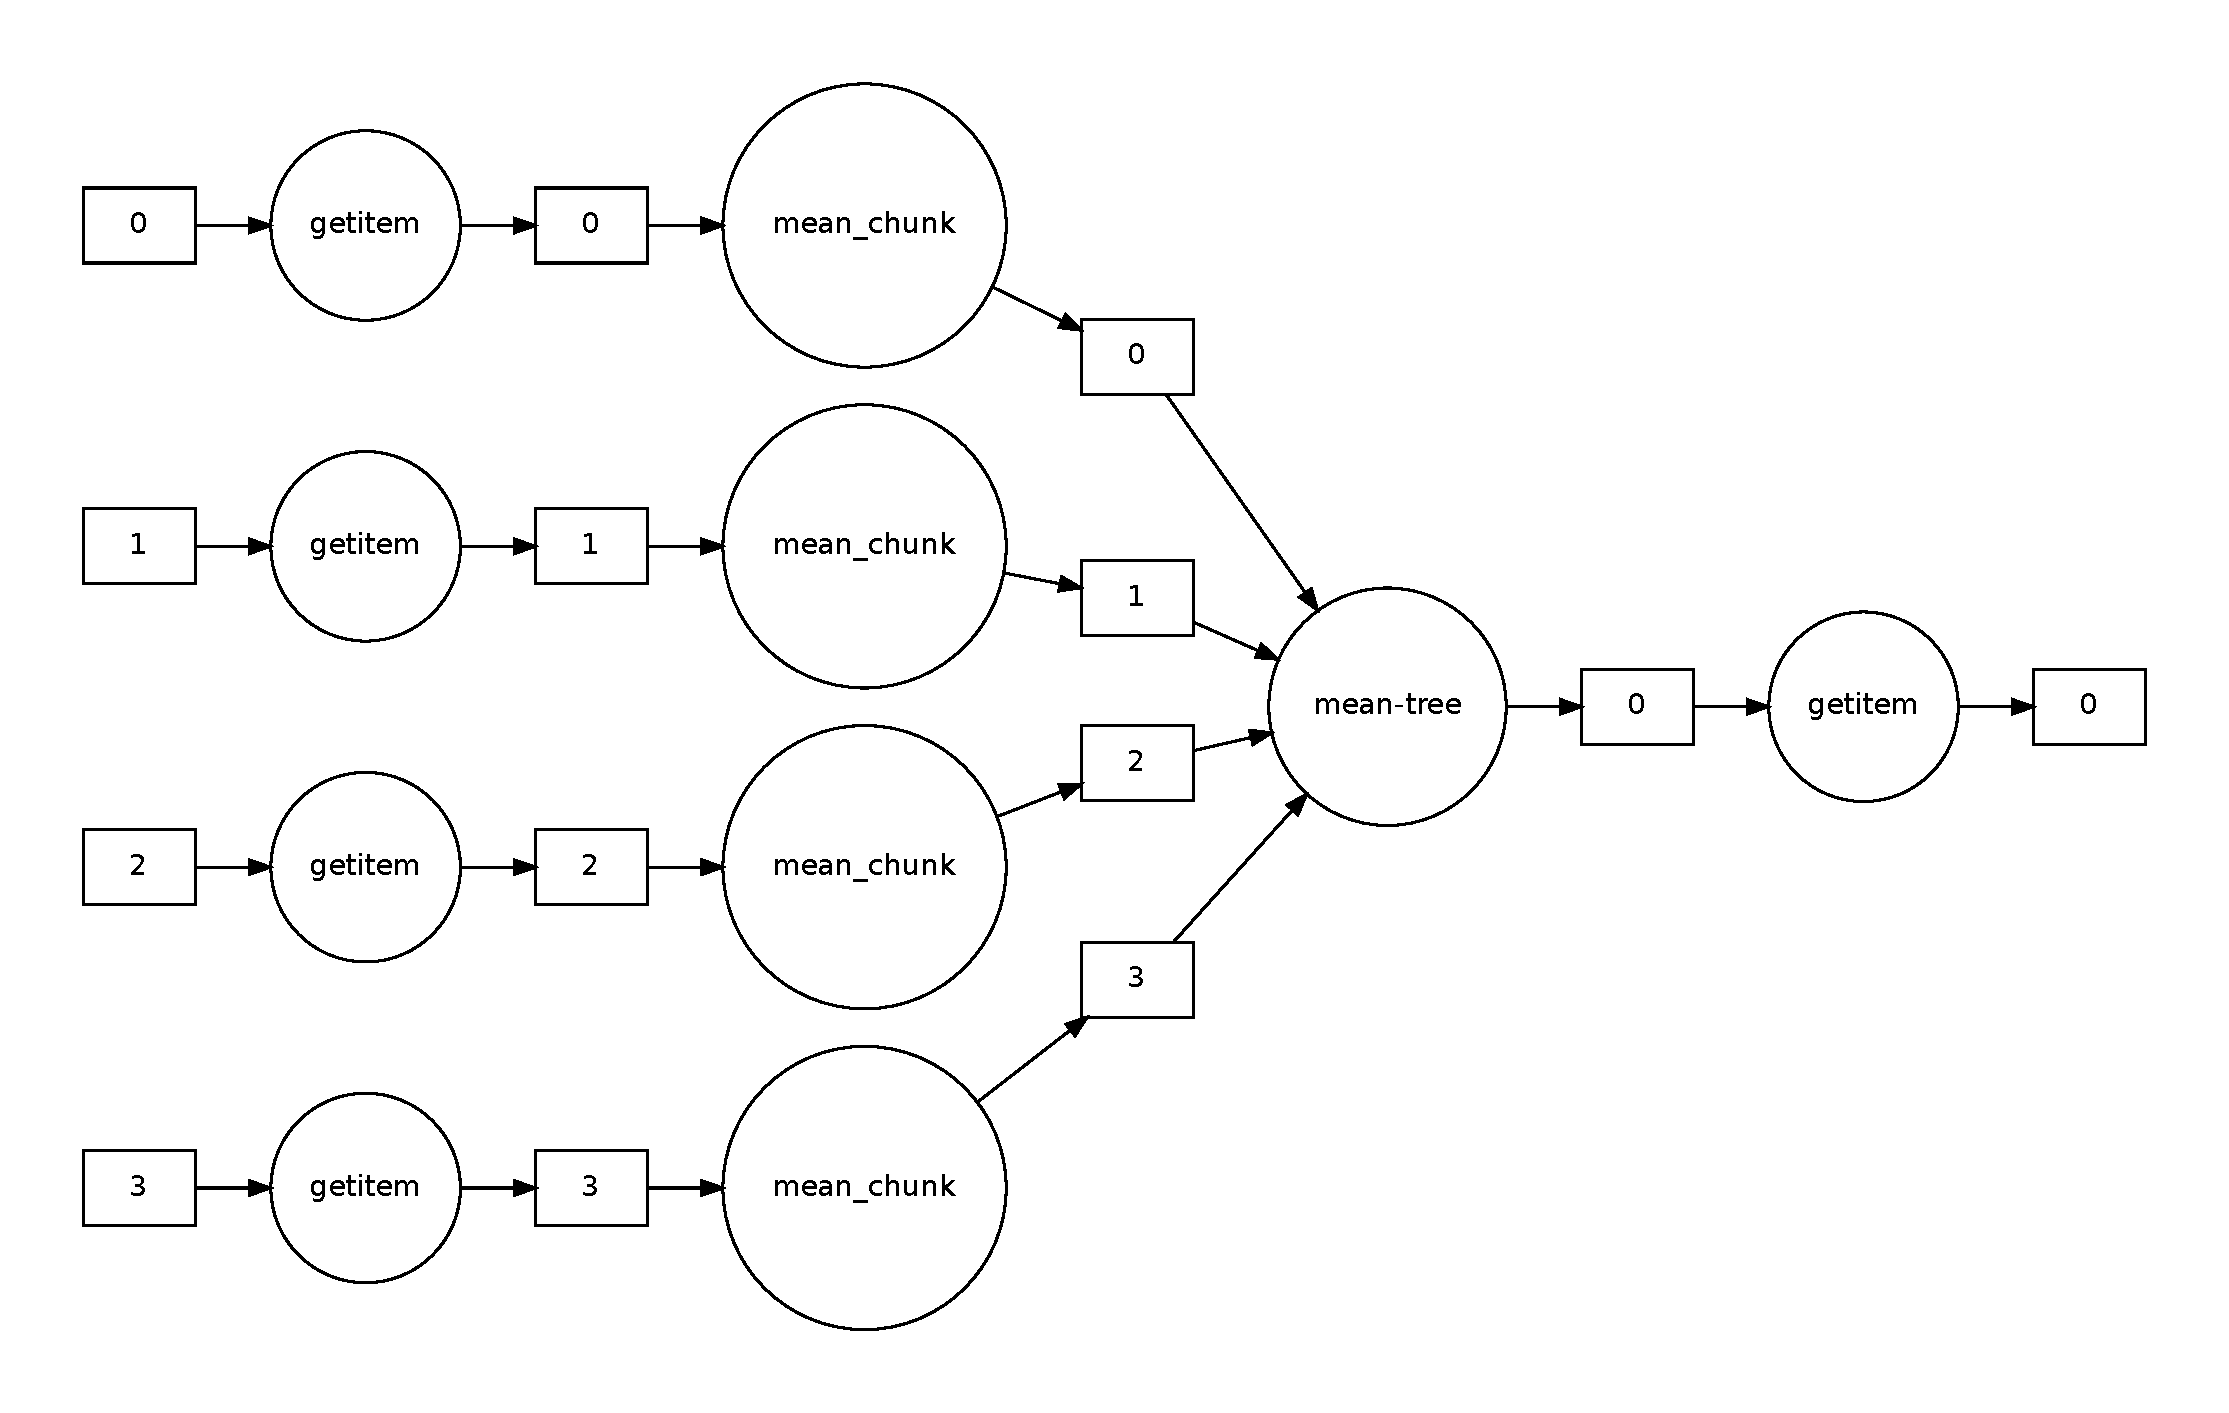
\includegraphics[width=\linewidth]{imgs/dask-dataframe-1-graph}
	\end{minipage}
\end{listing}

Specialized types of task graphs are also commonly used to parallelize \emph{dataframe}
processing, which is a popular approach for performing exploratory data analytics and
\gls{olap} queries over two-dimensional tabular datasets (dataframes). Tools such
as \dask{} DataFrame~\cite{dask},
Modin~\cite{modin}, Vaex~\cite{vaex} or
CuDF~\cite{cudf} offer e.g.\ Python \glspl{api} or
\gls{sql} interfaces for expressing queries over dataframes, and then translate
these queries into task graphs that are executed on parallel machines, distributed clusters or
\gls{gpu} accelerators. Users of these tools do not even necessarily have to know
that they are interacting with task graphs, since their usage is mostly an internal implementation
detail. \Autoref{lst:dask-dataframe-example-1} shows a short Python program that leverages the
\dask{} DataFrame \gls{api} for performing a query on a
dataframe loaded from a \gls{csv} file. The query is internally translated by
\dask{} to the task graph shown on the right side of the figure, which can then
be executed e.g.\ on a distributed cluster.

While MapReduce, DataFrame processing or other similar models are useful for computations that have
a predictable structure, they are not always general enough to express complex
\gls{hpc} scientific workflows. We will thus further only consider tools and
models that allow executing arbitrary task graphs. Note that especially DataFrame processing is
often used inside scientific workflows, but it typically represents only a certain part of the
workflow (e.g.\ a single task or a set of tasks), and it is not used to define the structure of the
whole workflow.

\subsection*{Task granularity}
Another important aspect of tasks is their \emph{granularity}. It is based on how much
work the task performs, and it also determines into how many subtasks it could be potentially
divided. In the extreme case, a \emph{coarse-grained} (low granularity) task could represent the whole
computation that we want to perform, while a \emph{fine-grained} (high granularity) task could represent only
the execution of a single \gls{cpu} instruction. With an increasing granularity,
the task performs less work, and the whole computation will thus have to be divided into a larger
number of tasks. This makes it easier to parallelize the computational workflow, yet it also
increases the overall overhead introduced by the task runtime, which has to manage and schedule
more tasks. The same properties also apply vice versa for a decreasing granularity of tasks.

Since tasks can represent arbitrary computations, it is not always straightforward to determine how
could they be subdivided into multiple tasks based on their structure, and therefore how granular
they are. Usually, it is much simpler to use a proxy metric for task granularity, based on the
duration that it takes to execute a task. Therefore, if a task is very fast to execute, we will
consider that it is highly granular, while if a task takes a long time to execute, we will consider
that it has low granularity.

Task granularity is important primarily because it determines how efficiently can a task graph be
parallelized and if it even makes sense to distribute it to multiple nodes at all. For example, if
certain tasks would take mere nanoseconds to execute, there would be no point in dynamically
load-balancing them across multiple distributed nodes, because the overhead of doing so would dwarf
the execution time of the tasks themselves, due to the latency induced by the network
communication. In other words, it would be faster to just execute all such tasks on the local node,
rather than sending them across the network. It could still be worth it to distribute a large
number of such extremely granular tasks to multiple nodes, but the distribution would need to
happen in an amortized way, for example only once at the beginning of the computation, to avoid the
excessive overhead.

Some task-based programming models focus primarily on high granularity tasks, for example
StarPU~\cite{starpu}, Cilk~\cite{cilk},
HPX~\cite{hpx}, PaRSEC~\cite{parsec},
Legion~\cite{legion}, TBB~\cite{tbb} or
\gls{openmp}~\cite{openmp}\footnote{Note that even though \gls{openmp} has been previously presented as an example of an
explicitly parallel model, it also offers a task system that provides facilities for implicit parallelization.}. In these
models, which are sometimes called \emph{task parallel}, tasks usually represent either
functions or blocks of code that contain a handful of instructions, and are typically relatively
quick to execute (they can run e.g.\ for milliseconds or seconds). While some of these tools also
support distributed computing, their main use-case is to provide intra-node parallelization on
multicore systems with shared memory, and often also to offload computation to attached
accelerators, such as \glspl{gpu} or \glspl{fpga}.

They can be used e.g.\ to implement high-performance numerically intensive computational kernels,
such as matrix multiplication or QR factorization~\cite{qr_factorization}, or to parallelize
recursive algorithms or algorithms with irregular data access patterns. \Autoref{lst:cilk-fibonacci}
shows a program implemented in the Cilk programming language, which calculates the n-th Fibonacci
number using a task parallel approach.

\begin{listing}
	\caption{Task-parallel Fibonacci calculation using Cilk\\Example adapted from~\cite{cilk}.}
	\label{lst:cilk-fibonacci}
	\begin{minted}[fontsize=\small, tabsize=4]{c}
cilk int fibonacci(int n)
{
	if (n < 2) {
		return n;
	}
	else
	{
		// Spawn a new task for each recursive call
		int x = spawn fibonaccib(n - 1);
		int y = spawn fibonaccib(n - 2);
		// Wait until the tasks finish with a barrier
		sync;
		return x + y;
	}
}
	\end{minted}
\end{listing}

Task parallel models definitely have their place in \gls{hpc}, however they are
not primarily designed for executing complex scientific workflows, therefore they are not the
primary focus of this thesis. Instead, we will mainly examine task-based programming models that
are designed for distributed execution on a cluster, with tasks whose duration typically spans from
milliseconds to hours or even days. The following section describes several state-of-the-art batch
processing distributed task runtimes.

\section{Distributed task runtimes}
There is a large body of tools designed for executing arbitrary task graphs on diverse computing
platforms, ranging from consumer-grade laptops, through cloud deployments, to distributed and
\gls{hpc} clusters. They are known under various terms, such as workflow
management systems, job managers, distributed job schedulers or orchestrators. We will use the term
\emph{task runtime} for all such task execution tools in this thesis. Examples of such task
runtimes include e.g.\ \dask{}~\cite{dask},
Parsl~\cite{parsl}, Ray~\cite{ray},
PyCOMPSs~\cite{pycompss}, HyperLoom~\cite{hyperloom},
Pydra~\cite{pydra}, Snakemake~\cite{snakemake},
SciLuigi~\cite{sciluigi}, Merlin~\cite{merlin},
Autosubmit~\cite{autosubmit}, NextFlow~\cite{nextflow},
StreamFlow~\cite{streamflow}, AiiDA~\cite{aiida},
FireWorks~\cite{fireworks} or Apache Airflow~\cite{airfow}. Each task
runtime defines its own instance of a task-based programming model, and has a different set of
trade-offs in areas such as performance and scalability, fault tolerance, data
provenance, ease-of-use, ease-of-deployment and others.

Since this thesis focuses on the ergonomics and performance aspects of executing task graphs on \gls{hpc} clusters,
this section discusses various challenges, bottlenecks and shortcomings that arise when the task
existing


However, as any programming model, it also has some disadvantages and problems. It is crucial to
understand these limitations in order to design approaches for overcoming them. This chapter thus
describes various challenges and requirements of this programing model, both in terms of efficient
and scalable execution, and in terms of the offered productivity and ergonomics. It focuses
specifically on challenges and requirements required by \gls{hpc} use-cases,
which introduce a unique set of constraints stemming both from the inherent complexity of
\gls{hpc} software and hardware and also from the sheer computational scale
required to efficiently utilize \gls{hpc} resources.

In addition to the challenges, we will also mention various desired properties and features which
should be offered by task runtimes in order to either support the mentioned requirements or to
alleviate the mentioned problems.

- architecture
- language/DSL/YAML/CWL

%Taxonomy - https://link.springer.com/article/10.1007/s11227-018-2238-4 - HyperShell
%(https://hyper-shell.readthedocs.io/en/latest/index.html) - flux - parsl - legate - pygion - dask -
%ray - snakemake - merlin - luigi - autosubmit - airflow -
%https://materialsproject.github.io/fireworks/ - pydra - (take more from references)

% TODO: https://docs.google.com/document/d/1C43tAGIRqy1hDHajRTiyM2q_TeihJwH0e66ASeGOwfU/edit#heading=h.rzzu2ckt23ak

\cite{task_based_taxonomy}

\subsection{Allocation manager}
\label{sec:allocation-manager}
Users of \gls{hpc} clusters are not typically allowed to directly perform
arbitrary computations on the computational nodes (machines designed to perform expensive
\gls{hpc} computations) of the cluster. Instead, they can connect to machines
that are usually called \emph{login nodes}, from where they have to enqueue their desired
computation into a queue handled by a submission system that manages the hardware resources of the
cluster and user accounting. We will use the term \emph{allocation manager} for these submission
systems, and the term \emph{allocation}\footnote{The term \emph{job} is also commonly used for the concept of
\gls{hpc} computational requests. However, this term will be used for a different concept described later in the thesis, therefore we use \emph{allocation} instead.} for a computational
request submitted by a user into the allocation manager. The majority of
\gls{hpc} clusters~\cite{slurm-schedmd} use one of the two most popular
allocation managers, either \gls{pbs}~\cite{pbs} or
Slurm~\cite{slurm}).

Each allocation states (amongst other things) the desired computational resources that the user
wants to utilize, primarily how many nodes they want to allocate, and what is the expected maximum
duration of their computation. The allocation is then submitted into a \emph{queue}
and starts executing only once there are enough free computational resources. Allocation managers
provide fair access to the cluster resources, to avoid their oversubscription and also to handle
accounting of the used resources. They tend to have fairly strict limits on the number of
allocations that users can submit and the number of nodes that they can have reserved for their
allocations at any given time. Because of these limits, allocations tend to be quite
coarse-grained. They typically ask for a whole node at minimum, and usually run at least for
minutes, but more typically hours or even days.

Since users have to create allocations to compute anything on the cluster, and thus they cannot
simply execute their task graphs directly, a question naturally arises -- how to map tasks (or task
graphs) to allocations in a way that will efficiently utilize \gls{hpc}
resources? Several ways of performing this task-to-allocation mapping are described below, however
all of them come with significant disadvantages.

\subsubsection*{Execute the whole task graph in a single allocation}
The simplest situation is when a task graph can be executed with a single allocation. If it does
not have a large number of tasks, or if it can be executed relatively quickly, users can create an
allocation that will compute the whole task graph. This approach is quite simple for the user,
since they just execute the task graph using a task runtime in the same way as they would on a
cluster without an allocation manager, or on a personal computer. The only difference is that they
have to define and submit an allocation that will bootstrap the computation.

However, since allocations are bound both by node count and a time limit, this approach is only
usable for rather small task graphs. Indeed, if the computation is short, it might not even make
sense to use an \gls{hpc} cluster to compute it. A more realistic scenario is
that even if an individual task graph can be executed quickly, users might want to execute many
such task graphs (for example to execute many experiments with different parametrizations). This
situation can be seen as a special case of a large task graph that consists of many disjoint
components (smaller task subgraphs). In this case, it will typically not be possible to execute all
such task graphs inside a single allocation.

\subsubsection*{Execute each task as an individual allocation}
From a certain point of view, \gls{hpc} allocation managers can also be viewed as
task runtimes that operate on a very coarse level -- their tasks being allocations that potentially
span hundreds of nodes, run for days or even longer and consist of many different program
executions. Ideally, there would be no difference between an allocation manager and a task runtime,
and users would just be able to construct an arbitrarily granular task graph and execute it
directly on an \gls{hpc} cluster in a straightforward way.

% https://rse.princeton.edu/2020/01/monitoring-slurm-efficiency-with-reportseff/
While this approach can certainly look tempting, in practice it is not usually feasible to use the
currently popular allocation managers (\gls{pbs} and Slurm) in this way, because
they operate on a level that is far too coarse for complex task graphs. While they do support
expressing dependencies between individual allocations in a crude way, they tend to have large
overhead per each allocation\todo[inline]{cite}, which can be several orders of magnitude
larger than for typical task runtimes (e.g.\ seconds vs milliseconds). Furthermore, they seldom
allow the user to create more than a few hundreds of allocations at the same time, both to provide
fairness and also because they simply cannot scale to such a number of allocations.

It should be noted that even though there is definitely room for improving the performance of
\gls{hpc} allocation managers, some of their complexity and performance
limitations are inherent. They have to provide accurate accounting, handle robust and secure
cleanup of hardware resource sprovided to allocations, manage user and process isolation on the
computational nodes, ensure user fairness and many other things. Many of these responsibilities are
out of scope for task runtimes, which enables them to achieve higher performance.

Another problem is node granularity. For ``small'' tasks that only use e.g.\ a few cores, users
would like to schedule and execute multiple tasks on a single node at the same time, to leverage
the available hardware resources efficiently. While allocation managers are able to create
allocations that require only a fraction of a node, this functionality is not always available.
Either for security reasons, because tasks from multiple users can then run on the same node at the
same time, which reduces user isolation, or for performance reasons, because the overhead of
scheduling a large number of allocations (in theory many allocations per each node) can become
unmanageable for the allocation manager~\cite{it4i_node_scheduling_policy}. When the manager is configured
in a way that a single allocation has to span at least a (complete) single node, it can lead to
wasted resources if a single task is unable to leverage the whole computational node.

Another reason why users might not want to use the allocation manager directly as a task runtime is
that it is useful to debug and prototype task graphs in a small-scale scenario (e.g.\ locally, on a
personal computer), before executing it on a large-scale \gls{hpc} system.
However, it can be quite challenging for users to deploy systems like \gls{pbs}
or Slurm locally. Therefore, they would need to use a different task runtime locally than on the
target \gls{hpc} platform, which woult not be very practical.

The mentioned issues stem from a dichotomy between the coarse-grained focused allocation manager
and more fine-grained focused task runtimes, which can create a barrier for
\gls{hpc} users. Users that want to execute a task graph on an
\gls{hpc} system thus usually use a separate task runtime (e.g.\
Dask~\cite{dask}) rather than using the allocation manager directly.

\subsubsection*{Partition the task graph into a smaller number of allocations}
The third approach that users may take is to partition their task graphs into smaller subgraphs,
and then submit each subgraph as a single allocation, where the subgraph will be computed by an
independent instance of a task runtime.

This is sort of an ultimate approach that the users will probably sooner or later converge to, once
their task graph becomes sufficiently complex and large, and they will have to somehow reconcile
the coarse-grained nature of allocations with the fine-grained nature of tasks and overcome the
overhead of creating too many allocations.

This process is not straightforward, especially if users have to perform the partitioning manually.
Graph partitioning itself is a notoriously difficult problem that is
NP-hard~\cite{graph_partitioning}\todo[inline]{Ada: Is this OK?}, and it is thus difficult to decide
beforehand how exactly should the task graph be split into allocations. Furthermore, if the
partitioning of tasks into allocations is performed statically, before the computation begins, then
it might lead to suboptimal hardware utilization, as it will not be possible to load-balance tasks
across different allocations, even if multiple allocations do run concurrently.

In addition to partitioning the task graph, this approach typically requires further implementation
efforts that are outside the boundaries of the task-based programming model. As an example, the
intermediate outputs of computed tasks of a partitioned subgraph might have to be persisted (to a
storage system) before the corresponding allocation ends, and the results from multiple allocations
then have to be merged together. In order to support recomputation of failed tasks, and submission
of new tasks while a task graph is already executing, it should also be possible to periodically
submit new allocations that could dynamically provide needed computational resources, until the
whole task graph is computed. This reduces the ergonomics of using task graphs, because it
basically requires users to reimplement parts of the task runtime behavior on top of the allocation
manager, in order to overcome its limitations.

\vspace{5mm}
The gap between allocation managers and task runtimes creates a disconnect for users attempting to
scale their task graph computation. Executing a task graph on a personal computer tends to be quite
simple. After that, moving to an \gls{hpc} cluster and executing the entire task
graph inside a single allocation is also quite straightforward. But once the task graph has to be
partitioned into multiple allocations, the simple abstraction of implicitly parallel task graphs
that can be executed with a single command quickly falls apart, as the user has to perform a lot of
additional work to make this scenario execute efficiently.

Ideally, users would not have to think about the allocation manager at all; they should be able to
construct a task graph and execute it directly on an \gls{hpc} cluster in a
straightforward way, by letting some tool perform the partitioning and load balancing across
allocations automatically for them. This could be achieved either by adding support for executing
fine-grained task graphs to allocation managers or by adding support for communicating with
allocation managers to task runtimes, to enable transparent execution of task graphs on
\gls{hpc} systems. This functionality is provided by several
\emph{meta-schedulers}, which will be mentioned in the next chapter.

\subsection{Cluster heterogeneity}
Even though task graphs are designed to be portable and ideally should not depend on any specific
execution environment, for certain types of tasks, we need to be able to describe at least some
generic environment constraints. For example, when a task executes a program that leverages the
CUDA\todo{explain} framework, which is designed to be executed on a graphics
accelerator, it has to be executed on a node that has a \gls{gpu} available,
otherwise it will simply not work.

It should thus be possible for an \gls{hpc} task to define
\emph{resource requirements}, which specify resources that have to be provided by an environment
that will execute such task. These requirements can be quite diverse. For example, a requirement
could be the number of cores (some tasks can use only a single core, some can be multithreaded),
the amount of available main memory, a minimum duration required to execute the task or (either
optional or required) presence of an accelerator like a \gls{gpu} or an
\gls{fpga}\@. In order to remain portable and independent of a specific execution
environment, these requirements should be abstract and describe general, rather than specific,
types of resources.

The challenge related to resource requirements of \gls{hpc} tasks specifically is
the diverse hardware present in modern \gls{hpc} clusters, which have started to
become increasingly heterogeneous in recent years. This trend can be clearly seen in the TOP500
list of most powerful supercomputers~\cite{top500analysis}. Individual cluster nodes contain
varying amounts and types of cores and sockets, main memory, \gls{numa} nodes or
accelerators like \glspl{gpu} or \glspl{fpga}. Since
\gls{hpc} software tries to leverage all these modern \gls{hpc}
hardware features, this complexity is also propagated to tasks and their resource requirements,
which can become relatively complex.

Some types of tasks might require a combination of several requirements, for example two
\glspl{gpu}, sixteen cores and 32 GiB of main memory. Some tasks are designed in a
way that allows them to leverage an open-ended range of resources, e.g.\ a task might require four
cores, but if more are available, it could use as many as possible. Furthermore, some tasks might
even support several variants of requirements, for example a task might either use four cores and a
single \gls{gpu} (if there is one available), or it could use more cores (and no \gls{gpu})
to offset the absence of an accelerator.

A resource requirement that is fairly specific to \gls{hpc} systems is the
requirement of using multiple nodes per single task. This requirement is necessary for programs
that are designed to be executed in a distributed fashion, such as programs using
\gls{mpi}, which are quite common in \gls{hpc}. This
requirement is not supported in many task runtimes, because their programming model assumes that a
task performs an atomic computation that executes on a single node. The use-case of tasks using
multiple nodes is discussed in more detail later in this chapter.

To support the mentioned scenarios, task runtimes should allow users to specify arbitrarily
fine-grained and abstract resource requirements for each task. They should also allow users to
attach resources that will satisfy these requirements to each individual instance of an execution
environment that will execute the tasks. Runtimes should also be able to take these requirements
into account when scheduling, both to make sure that the requirements are upheld, and also to
utilize the available hardware effectively.

\subsection{Data transfers}
After a task is computed, it can produce various data outputs, standard error or output streams,
files created on the disk or data objects that are then passed as inputs to dependent tasks. There
are many ways of storing and transferring these outputs. Some task frameworks store task outputs on
the filesystem, since it is relatively simple to implement, and it provides support for basic data
resiliency out-of-the-box.

\gls{hpc} nodes might not contain any local disks, but instead use shared
filesystems accessed over a network. While this can be seen as an advantage, since with a shared
filesystem it is much easier to share task outputs amongst different workers, it can also be a
severe bottleneck. Shared networked filesystems can suffer from quite high latency, and accessing
them can consume precious network bandwidth that is also used e.g.\ for managing computation
(sending commands to workers) or for direct worker-to-worker data exchange. Furthermore, data
produced in \gls{hpc} computations can be quite large, and thus storing it to a
disk can be a bottleneck even without considering networked filesystems.

These bottlenecks can be alleviated by transferring task outputs directly between workers over the
network (preferably without accessing the filesystem in the fast path), by streaming outputs
between tasks without the need to store them or by leveraging \gls{ram}
disks~\cite{hyperloom}. Making use of \gls{hpc} specific technologies,
such as \gls{mpi} or InfiniBand, could be also worthwhile to leverage the very
fast interconnects available in \gls{hpc} clusters.

Data outputs produced by tasks tend to be considered immutable in existing task runtimes, since a
single output can be used as an input to multiple tasks, and these might be executed on completely
different computational nodes. A problem that can arise with this approach is that if the data
outputs are large, but the computation within tasks that work with the data is short, the
serialization overhead (or even memory copy overhead, if the dependent task is executed on the same
node) can dominate the execution time. Such use-cases can be solved with stateful data management,
for example in the form of \emph{actors}, which can be considered stateful tasks that
operate on a single copy of some large piece of data.

\subsection{Fault tolerance}
Fault tolerance is relevant in all distributed computing environments, but
\gls{hpc} systems have specific requirements in this regard. As was already
mentioned, computational resources on \gls{hpc} clusters are provided through
allocation managers. Computing nodes allocated by these managers are provided only for a limited
duration, which means that for long-running task graphs, some nodes will disconnect and new nodes
will appear dynamically during the execution of the task graph. Furthermore, since the allocations
go through a queue, it can take some time before new computational resources arrive, therefore the
task graph can remain in a paused state, where no tasks are being executed, for potentially long
periods of time.

It is important for task runtimes to be prepared for these situations; they must handle node
disconnections gracefully, even if a task was being executed on a node that disconnects, and they
should be able to restart previously interrupted tasks on newly arrived workers. In general, in
\gls{hpc} scenarios, worker instability and frequent disconnects should be
considered the norm, not just a rare edge case.

\subsection{Multi-node tasks}
Many existing \gls{hpc} applications are designed to be executed on multiple
(potentially hundreds or even thousands) nodes in parallel, using e.g.\ \gls{mpi}
libraries or other communication frameworks. Multi-node execution could be seen as a special
resource requirement, which states that a task should be executed on multiple workers at once.

Support for multi-node tasks affects many design areas of a task runtime:
\begin{description}
	\item[Scheduling] When a task requires multiple nodes for execution and not enough nodes are available at a given
		moment, the scheduler has to decide on a strategy that will allow the multi-node task to execute.
		If it was constantly trying to backfill available workers with single-node tasks, the multi-node
		tasks could be starved.

		The scheduler might thus have to resort to keep some nodes idle for a while to enable the
		multi-node task to start as soon as possible. Another approach could be to interrupt the currently
		executing tasks and checkpoint their state to make space for a multi-node task, and then resume
		their execution once the multi-node task finishes.

		In a way, this decision-making already has to be performed on the level of individual cores even
		for single-node tasks, but adding multiple nodes per task makes the problem much more difficult.
	\item[Data transfers] It is relatively straightforward to express data transfers between single-node tasks in a task
		graph, because they naturally correspond to dependencies (edges) between the tasks. With multi-node
		tasks, the data distribution patterns become more complex, for example data can be replicated from
		a single node to multiple nodes when a multi-node task starts or gathered (reduced) from multiple
		nodes to a single node when such task finishes.

		When several multi-node tasks depend on one another, the task runtime should be able to exchange
		data between them in an efficient manner. This might require some cooperation with the used
		communication framework (e.g.\ \gls{mpi}) to avoid needless repeated serialization
		and deserialization.
	\item[Fault tolerance] When a node executing a single-node task crashes or disconnects from the runtime, its task can be
		rescheduled to a different worker. In the case of multi-node tasks, failure handling requires more
		communication and is generally more complex. When a task is executing on four nodes and one of them
		fails, the runtime has to make sure that the other nodes will be notified of this situation, so
		that they can react accordingly (either by finishing the task with a smaller number of nodes or by
		also failing immediately).
\end{description}

To enable common \gls{hpc} usecases, task runtimes should be able to provide some
support for multi-node tasks and allow them to be combined with single-node tasks. Advanced
multi-node task support could be provided e.g.\ by offering some kind of integration with
\gls{mpi} or similar common \gls{hpc} technologies.

\subsection{Scalability}
The sheer scale of \gls{hpc} performance (node count, core count, network
interconnect bandwidth) opens up opportunities for executing large scale task graphs, but that in
turn presents unique challenges for task runtimes. Below you can find several examples of
bottlenecks that might not matter in a small computational scale, but that can become problematic
in the context of \gls{hpc}-scale task graphs.

\begin{description}
	\item[Task graph materialization] Large computations might require building massive task graphs that contain millions of tasks. The
		task graphs are typically defined and built outside the task runtime itself, for example on the
		login nodes of computing clusters or on client devices (e.g.\ laptops), which can provide only
		relatively low performance. It can be quite slow to build, serialize and transfer such graphs over
		the network to the task runtime. This can create a bottleneck even before any task is executed.
		This has been identified as an issue in existing task runtimes~\cite{dask-client-perf}.

		In such case, it can be beneficial to provide an \gls{api} for defining task
		graphs in a symbolic way, for example by representing a potentially large group of similar tasks by
		a single entity. Such symbolic graphs could then be sent to the runtime in a compressed form and
		re-materialized only at the last possible moment. In an extreme form, the runtime could operate on
		such graphs in a fully symbolic way, without ever materializing them.
	\item[Communication overhead] Scaling the number of tasks and workers will necessarily put a lot of pressure on the communication
		network, both in terms of bandwidth (sending large task outputs between nodes) and latency (sending
		small management messages between the scheduler and the workers). Using \gls{hpc}
		technologies, such as \gls{mpi} or a lower-level interface like
		\gls{rdma}, could provide a non-trivial performance boost in this regard.

		As we have demonstrated in~\cite{pspin, spin2}, in-network computing, an active area of
		research, can be also used to optimize various networking applications by offloading some
		computations to an accelerated \gls{nic}. This approach could also be leveraged
		for task runtimes, for example by reducing the latency of management messages between the scheduler
		and workers or by increasing the bandwidth of large data exchanges amongst workers, by moving these
		operations directly onto the network card.
	\item[Runtime overhead] As we have shown in~\cite{rsds}, task runtimes with a centralized scheduler have to
		make sure that their overhead remains manageable. Even with an overhead of just
		$1ms$ per task, executing a task graph with a million tasks would result in
		total accumulated overhead of twenty minutes! Our results indicate that increasing the performance
		of the central scheduling and management component of a task runtime can have a large positive
		effect on the overall time it takes to execute the whole task graph.

		However, the performance of the central server cannot be increased endlessly, and from some point,
		using a centralized architecture, which is common to task runtimes, itself becomes a bottleneck.
		Even if the workers exchange large output data directly between themselves, any single, centralized
		component may become overloaded simply by coordinating and scheduling the workers.

		In that case, a decentralized architecture could be leveraged to avoid the reliance on a central
		component. Such a decentralized architecture can be found e.g.\ in Ray~\cite{ray}.
		However, to realize the gains of a decentralized architecture, task submission itself has to be
		decentralized in some way, which might not be a natural fit for common task graph workflows. If all
		tasks are generated from a single component, the bottleneck will most likely remain even in an
		otherwise fully decentralized system.
\end{description}

\subsection{Iterative computation}
A natural way of executing task graphs is to describe the whole computation with a single task
graph, submit the graph to the task runtime and wait until all the tasks are completed. However,
there are some computations that need a more iterative approach. Training a machine learning model
can be stopped early if the loss is no longer decreasing. A chemical or physical simulation is only
considered completed once a desired accuracy has been reached, which might take a previously
unknown number of steps. These scenarios and many others like them, are quite common in
\gls{hpc} use cases.

To support iterative computation, task runtimes should allow the user to stop the execution of a
task graph (or its subgraph) once a specific condition is met, and also to add new tasks to the
task graph in a dynamic fashion, if it is discovered that more iterations are needed.

\subsection{Deployment}
- Python is hard to deploy

\subsection{Summary}
Even though more \gls{hpc} use-cases and oddities could always be found, it is
already clear from the mentioned challenges that \gls{hpc} use-cases that
leverage task graphs can contain a lot of complexity. It could be possible to add support for some
mentioned requirements to existing task runtimes, which are described in the next section. However,
the described challenges are so diverse and complex that a dedicated approach which considers them
holistically could provide a better solution that would avoid both ergonomics and performance from
being compromised.

The aforementioned requirements will serve as a basis for further research in the proposed thesis.
The goal of the thesis is to design approaches for executing task graphs on
\gls{hpc} systems that take the aforementioned requirements into account. These
approaches will leverage the \hyperqueue{} task runtime, which is described further
in~\Autoref{ch:hyperqueue}.
